\begin{frame}{Results 1 - Both target BC (6 - 32 q)}
    
    \label{BCA_MBC}

    \vspace{-0.25cm}

    \begin{figure}
        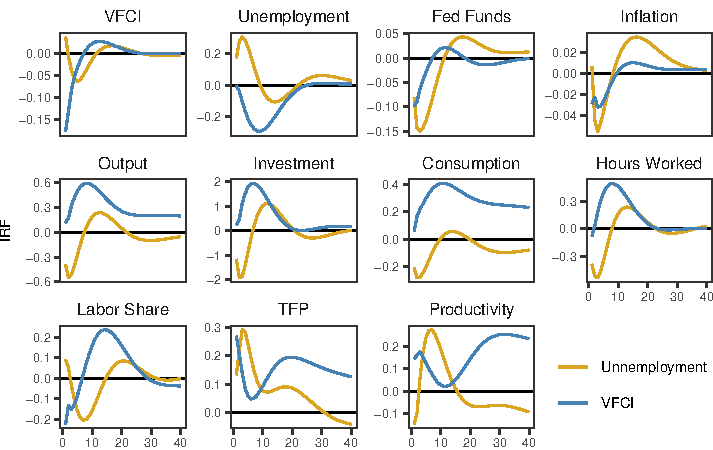
\includegraphics[height = 3in]{figs/fig3_BCA_MBC.pdf}
    \end{figure}

    \gotobutton{1.5}{0.3}{BCA_MBC_diff}{Differences}
    \gotobutton{3.25}{0.3}{BCA_MBC_first_diff}{First Differences}
\end{frame}



\begin{frame}{Results 2 - Both target 22 - 32 q}
    
    \label{results-2}

    \vspace{-0.25cm}

    \begin{figure}
        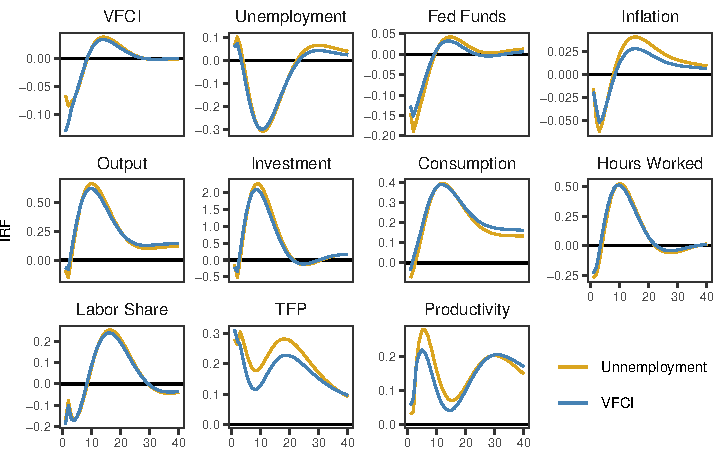
\includegraphics[height = 3in]{figs/fig5_vfci_u_same_freq.pdf}
    \end{figure}

\end{frame}


\begin{frame}{Results 3 - Residual of MBC }
    
    \label{results-3}

    \vspace{-0.25cm}

    \begin{figure}
        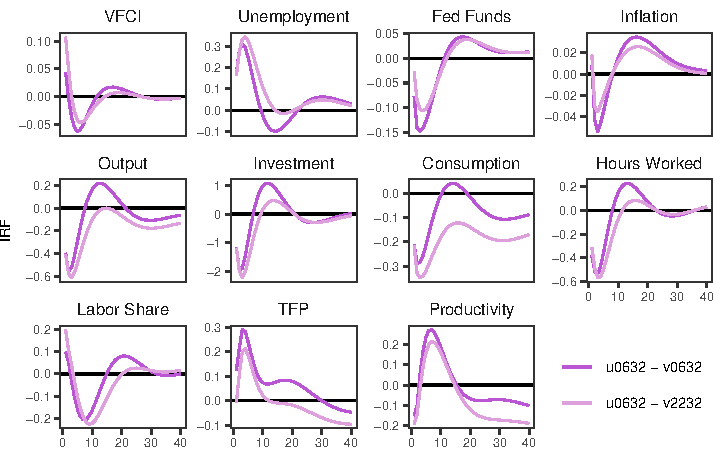
\includegraphics[height = 3in]{figs/fig6_resid_MBC.pdf}
    \end{figure}
    

\end{frame}


\begin{frame}{Rotation Weights }
    
    \vspace{-0.25cm}
    
    \begin{figure}
        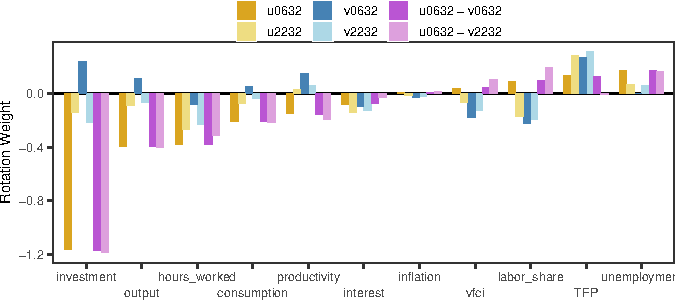
\includegraphics[height = 2in]{figs/fig7_weights.pdf}
    \end{figure}

\end{frame}

\begin{frame}{Empirical Shock Weights }
    
    \vspace{-0.25cm}
    
    \begin{figure}
        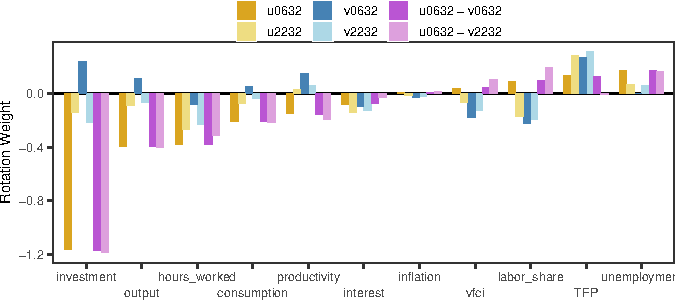
\includegraphics[height = 2in]{figs/fig11_emp_weights.pdf}
    \end{figure}

\end{frame}


\begin{frame}{Other - Historical Shocks }
    
    \vspace{-0.25cm}

    \begin{figure}
        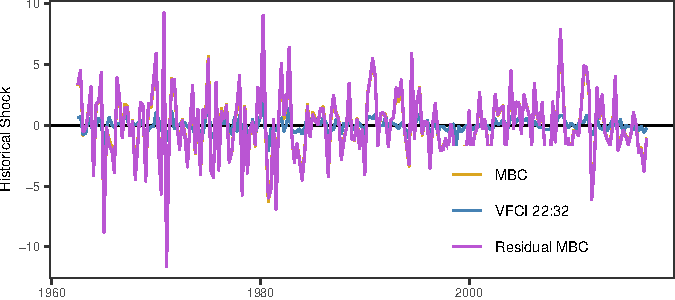
\includegraphics[height = 3in]{figs/fig8_hist_shocks.pdf}
    \end{figure}

\end{frame}


\begin{frame}{Other - FEVDFD }
    
    \vspace{-0.25cm}
    
    \begin{figure}
        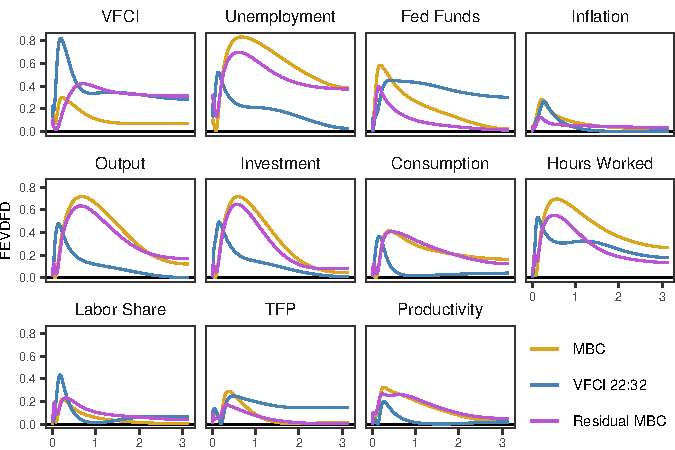
\includegraphics[height = 3in]{figs/fig9_fevdfd.pdf}
    \end{figure}

\end{frame}


\begin{frame}{Other - FEVD }
    
    \vspace{-0.25cm}
     
    \begin{figure}
        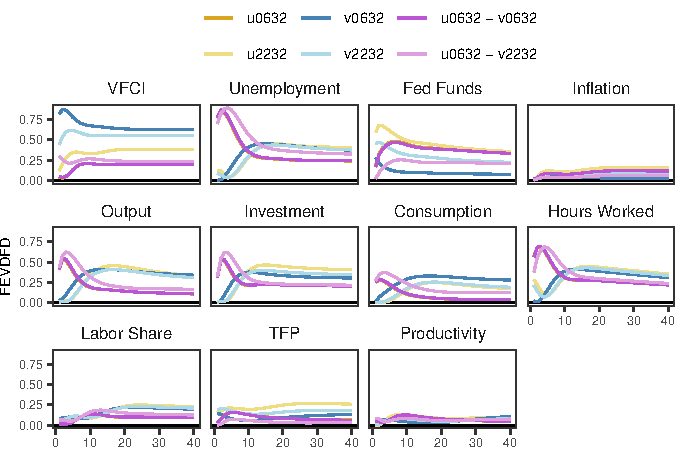
\includegraphics[height = 3in]{figs/fig10_fevd.pdf}
    \end{figure}   

\end{frame}